\begin{figure}[pt]
\centering
\arrayrulecolor{gray}
\resizebox{\linewidth}{!}{
\begin{tabular}{|p{\linewidth}|}
\hline\vspace{-0.5em}
\begin{minipage}[c]{\linewidth} 
\fig{xtree}.A: To determine which of  metrics are usually changed together, we use frequent itemset mining. Our dataset is continuous in nature (see (a)) so we first discretize  using Fayyad-Irani~\citep{fi}; this gives us a representation shown in (b). Next, we convert these into ``transactions'' where each file contains a list of discretized OO-metrics (see (c)). Then we use  the  {\em FP-growth} algorithm to mine frequent itemsets. We return the \textit{maximal frequent itemset} (as in (d)). Note: in (d) the row in \colorbox{lightgreen}{green} is the maximal frequent itemset.\\
\begin{minipage}[c]{\linewidth}
\begin{minipage}[c]{0.45\linewidth}
\resizebox{\linewidth}{!}{
\begin{tabular}{@{}c|c|c|c|c|c@{}}
    &rfc&loc&dit&cbo&Bugs  \\\hline
1.java&0.6&100&1&4&0  \\\hline
2.java&0.9&223&4&5&1  \\\hline
3.java&1.1&290&5&7&1  \\\hline
4.java&2.1&700&10&12&3  \\\hline
5.java&2.3&800&11&15&3  \\
\end{tabular}}
\end{minipage}$~~~\longrightarrow~~~$\begin{minipage}[c]{0.375\linewidth}
\resizebox{\linewidth}{!}{
\begin{tabular}{@{}c|c|c|c|c@{}}
    &rfc&loc&dit&cbo  \\\hline
1.java&A&A&A&A  \\\hline
2.java&A&A&B&A  \\\hline
3.java&A&A&B&A  \\\hline
4.java&B&B&C&B \\\hline
5.java&B&B&C&B  \\
\end{tabular}}
\end{minipage}
\end{minipage}
\begin{minipage}[c]{\linewidth}
\centering
(a)\hspace{0.5\linewidth}(b)
\end{minipage}
\begin{minipage}[c]{0.4\linewidth}
\resizebox{\linewidth}{!}{
\begin{tabular}{@{}c|c@{}}
    &Items  \\\hline
1.java&$rfc_A,~loc_A,~dit_A,~cbo_A$  \\\hline
2.java&$rfc_A,~loc_A,~dit_B,~cbo_A$  \\\hline
3.java&$rfc_A,~loc_A,~dit_B,~cbo_A$  \\\hline
4.java&$rfc_B,~loc_B,~dit_C,~cbo_B$  \\\hline
5.java&$rfc_B,~loc_B,~dit_C,~cbo_B$  \\
\end{tabular}}
\end{minipage}$~~~\longrightarrow~~~$\begin{minipage}[c]{0.45\linewidth}
\resizebox{\linewidth}{!}{
\begin{tabular}{@{}c|c@{}}
Items (\texttt{min\_sup=60})   & Support  \\\hline
$rfc_A$ & 60\\\hline
$loc_A$ & 60\\\hline
\st{$dit_A$} & \st{40}\\\hline
$\{rfc_A, loc_A\}$, $\{loc_A, cbo_A\}$, \ldots & 60 \\\hline
\rowcolor{lightgreen}$\{rfc_A, loc_A, cbo_A\}$&  60 \\\hline
\rowcolor{white}\st{$\{rfc_A, loc_A, cbo_A, dit_{B,C}\}$}&\st{40}   \\
\end{tabular}}
\end{minipage}
\begin{minipage}[c]{\linewidth}
\centering
(c)\hspace{0.5\linewidth}(d)
\end{minipage}\vspace{0.4em}
\end{minipage}\bigstrut\\\hline\vspace{-0.5em}
\begin{minipage}[c]{\linewidth}
\fig{xtree}.B: To build the decision tree, we find the most informative feature,i.e., the feature which has the lowest mean entropy of splits and construct a decision tree recursively in a top-down fashion as show below.\\
\begin{minipage}[c]{\linewidth}
\begin{minipage}[c]{0.5\textwidth}
\centering
    % 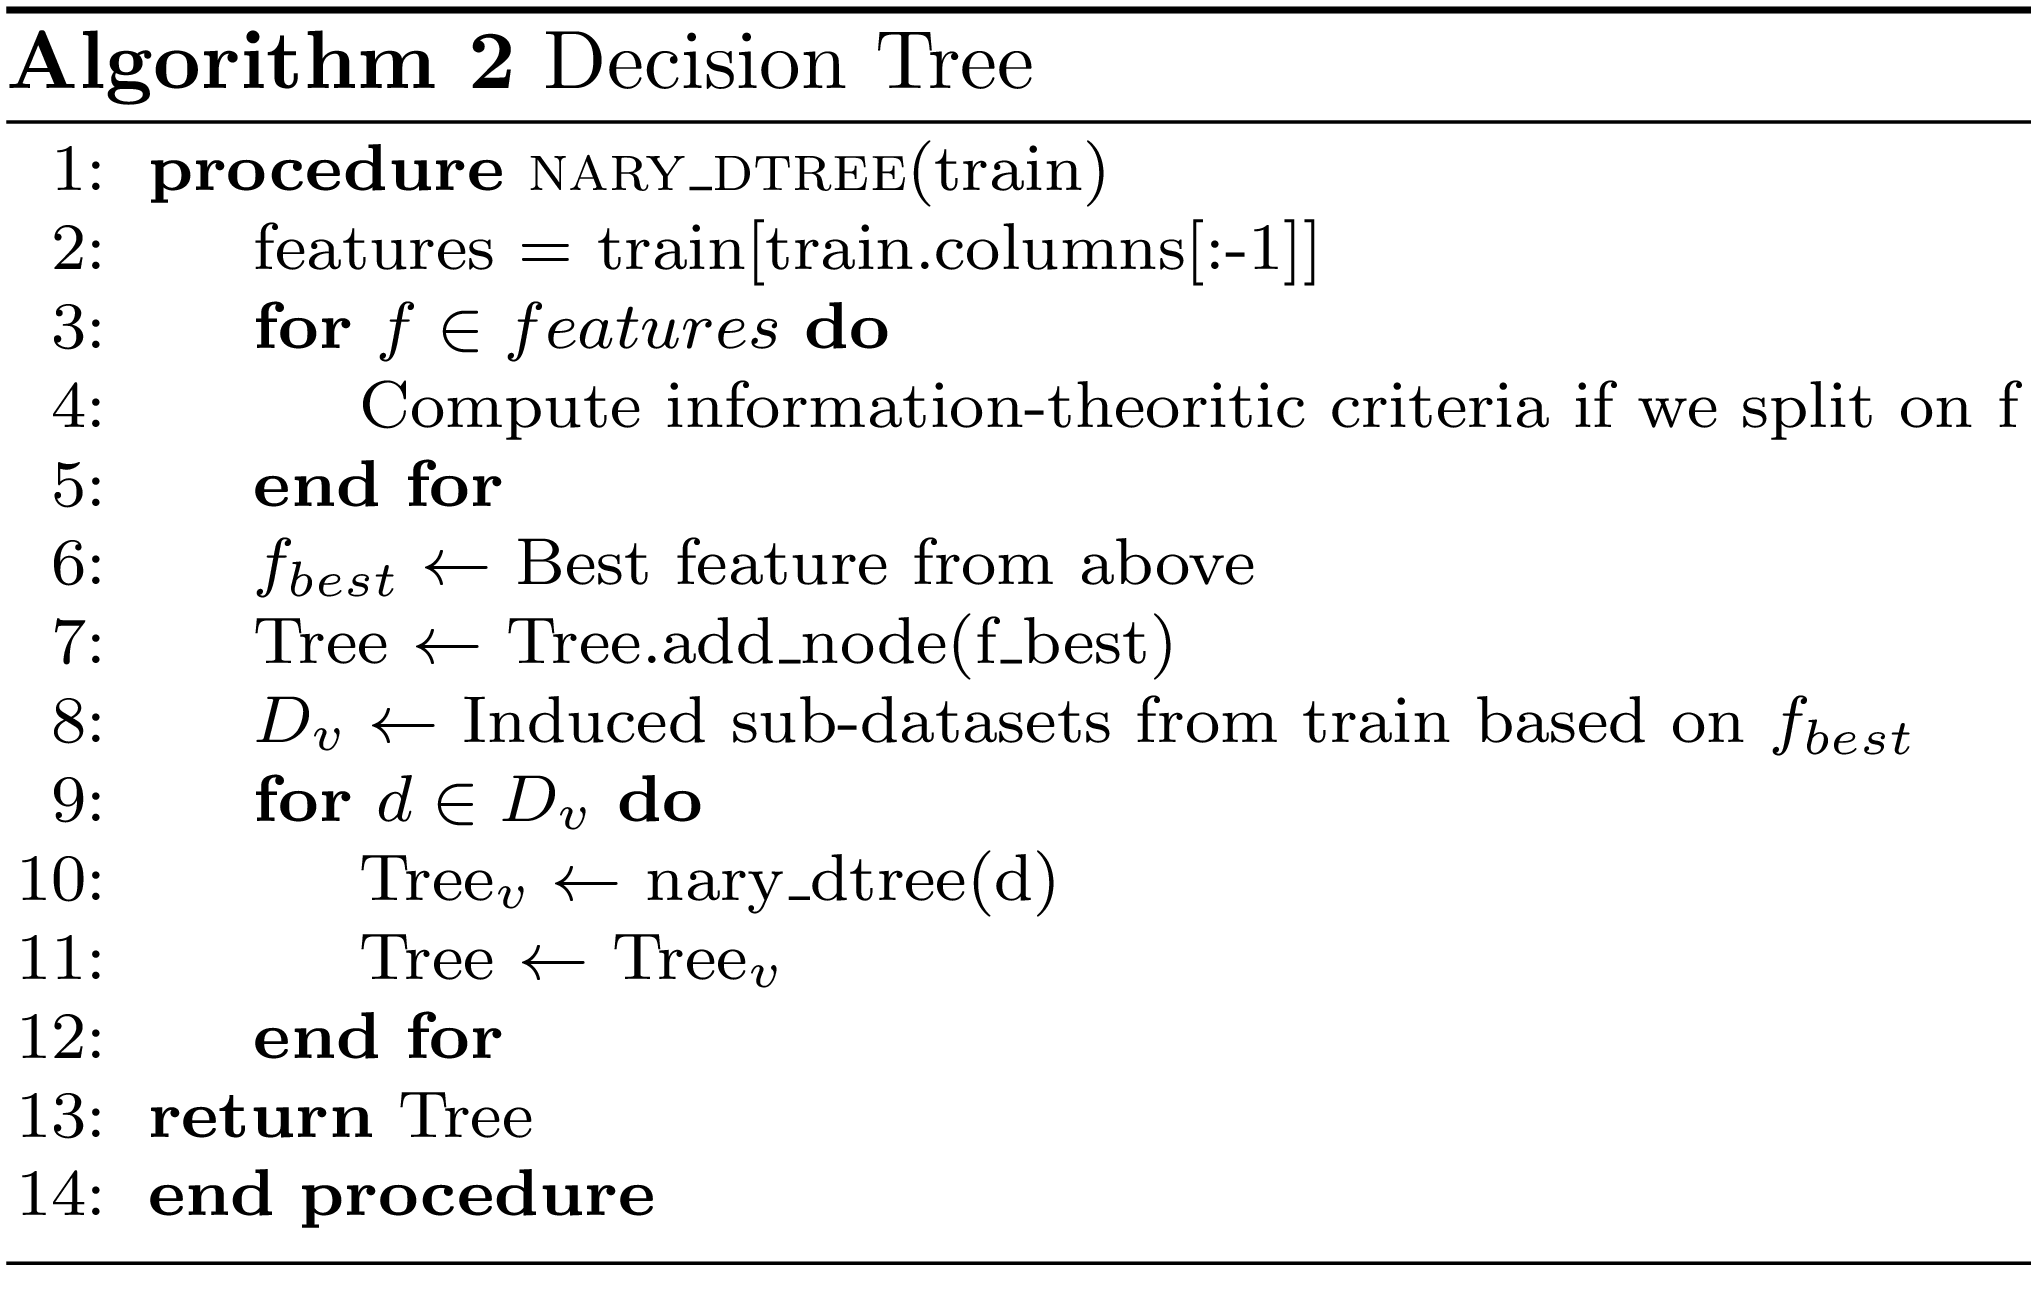
\includegraphics[width=\linewidth]{dtree_algo.png}
  \begin{algorithm}[H]\scriptsize
    \caption{N-ary Decision Tree}\label{alg:dtree}
    \begin{algorithmic}[0]
    \Procedure{nary\_dtree}{train}
    \State features = train[train.columns[:-1]]
    \For{$f \in features$}
        \State Find splits using Fayyad-Irani method
        \State Compute expected entropy of splits
    \EndFor
    \State $f_{best} \gets $ Feature with lowest mean entropy
    \State Tree $\gets$ Tree.\texttt{add\_node}(f\_best)
    \State $D_{v} \gets$ Induced sub-datasets from train based on $f_{best}$
     \For{$d \in D_{v}$}
        \State Tree$_v \gets$  \textsc{nary\_dtree}(d)
        \State Tree $\gets$ Tree$_v$
    \EndFor\\
    \noindent\Return Tree
    \EndProcedure
    \end{algorithmic}
 \end{algorithm}
\end{minipage}~\begin{minipage}[c]{0.475\textwidth}
\centering
    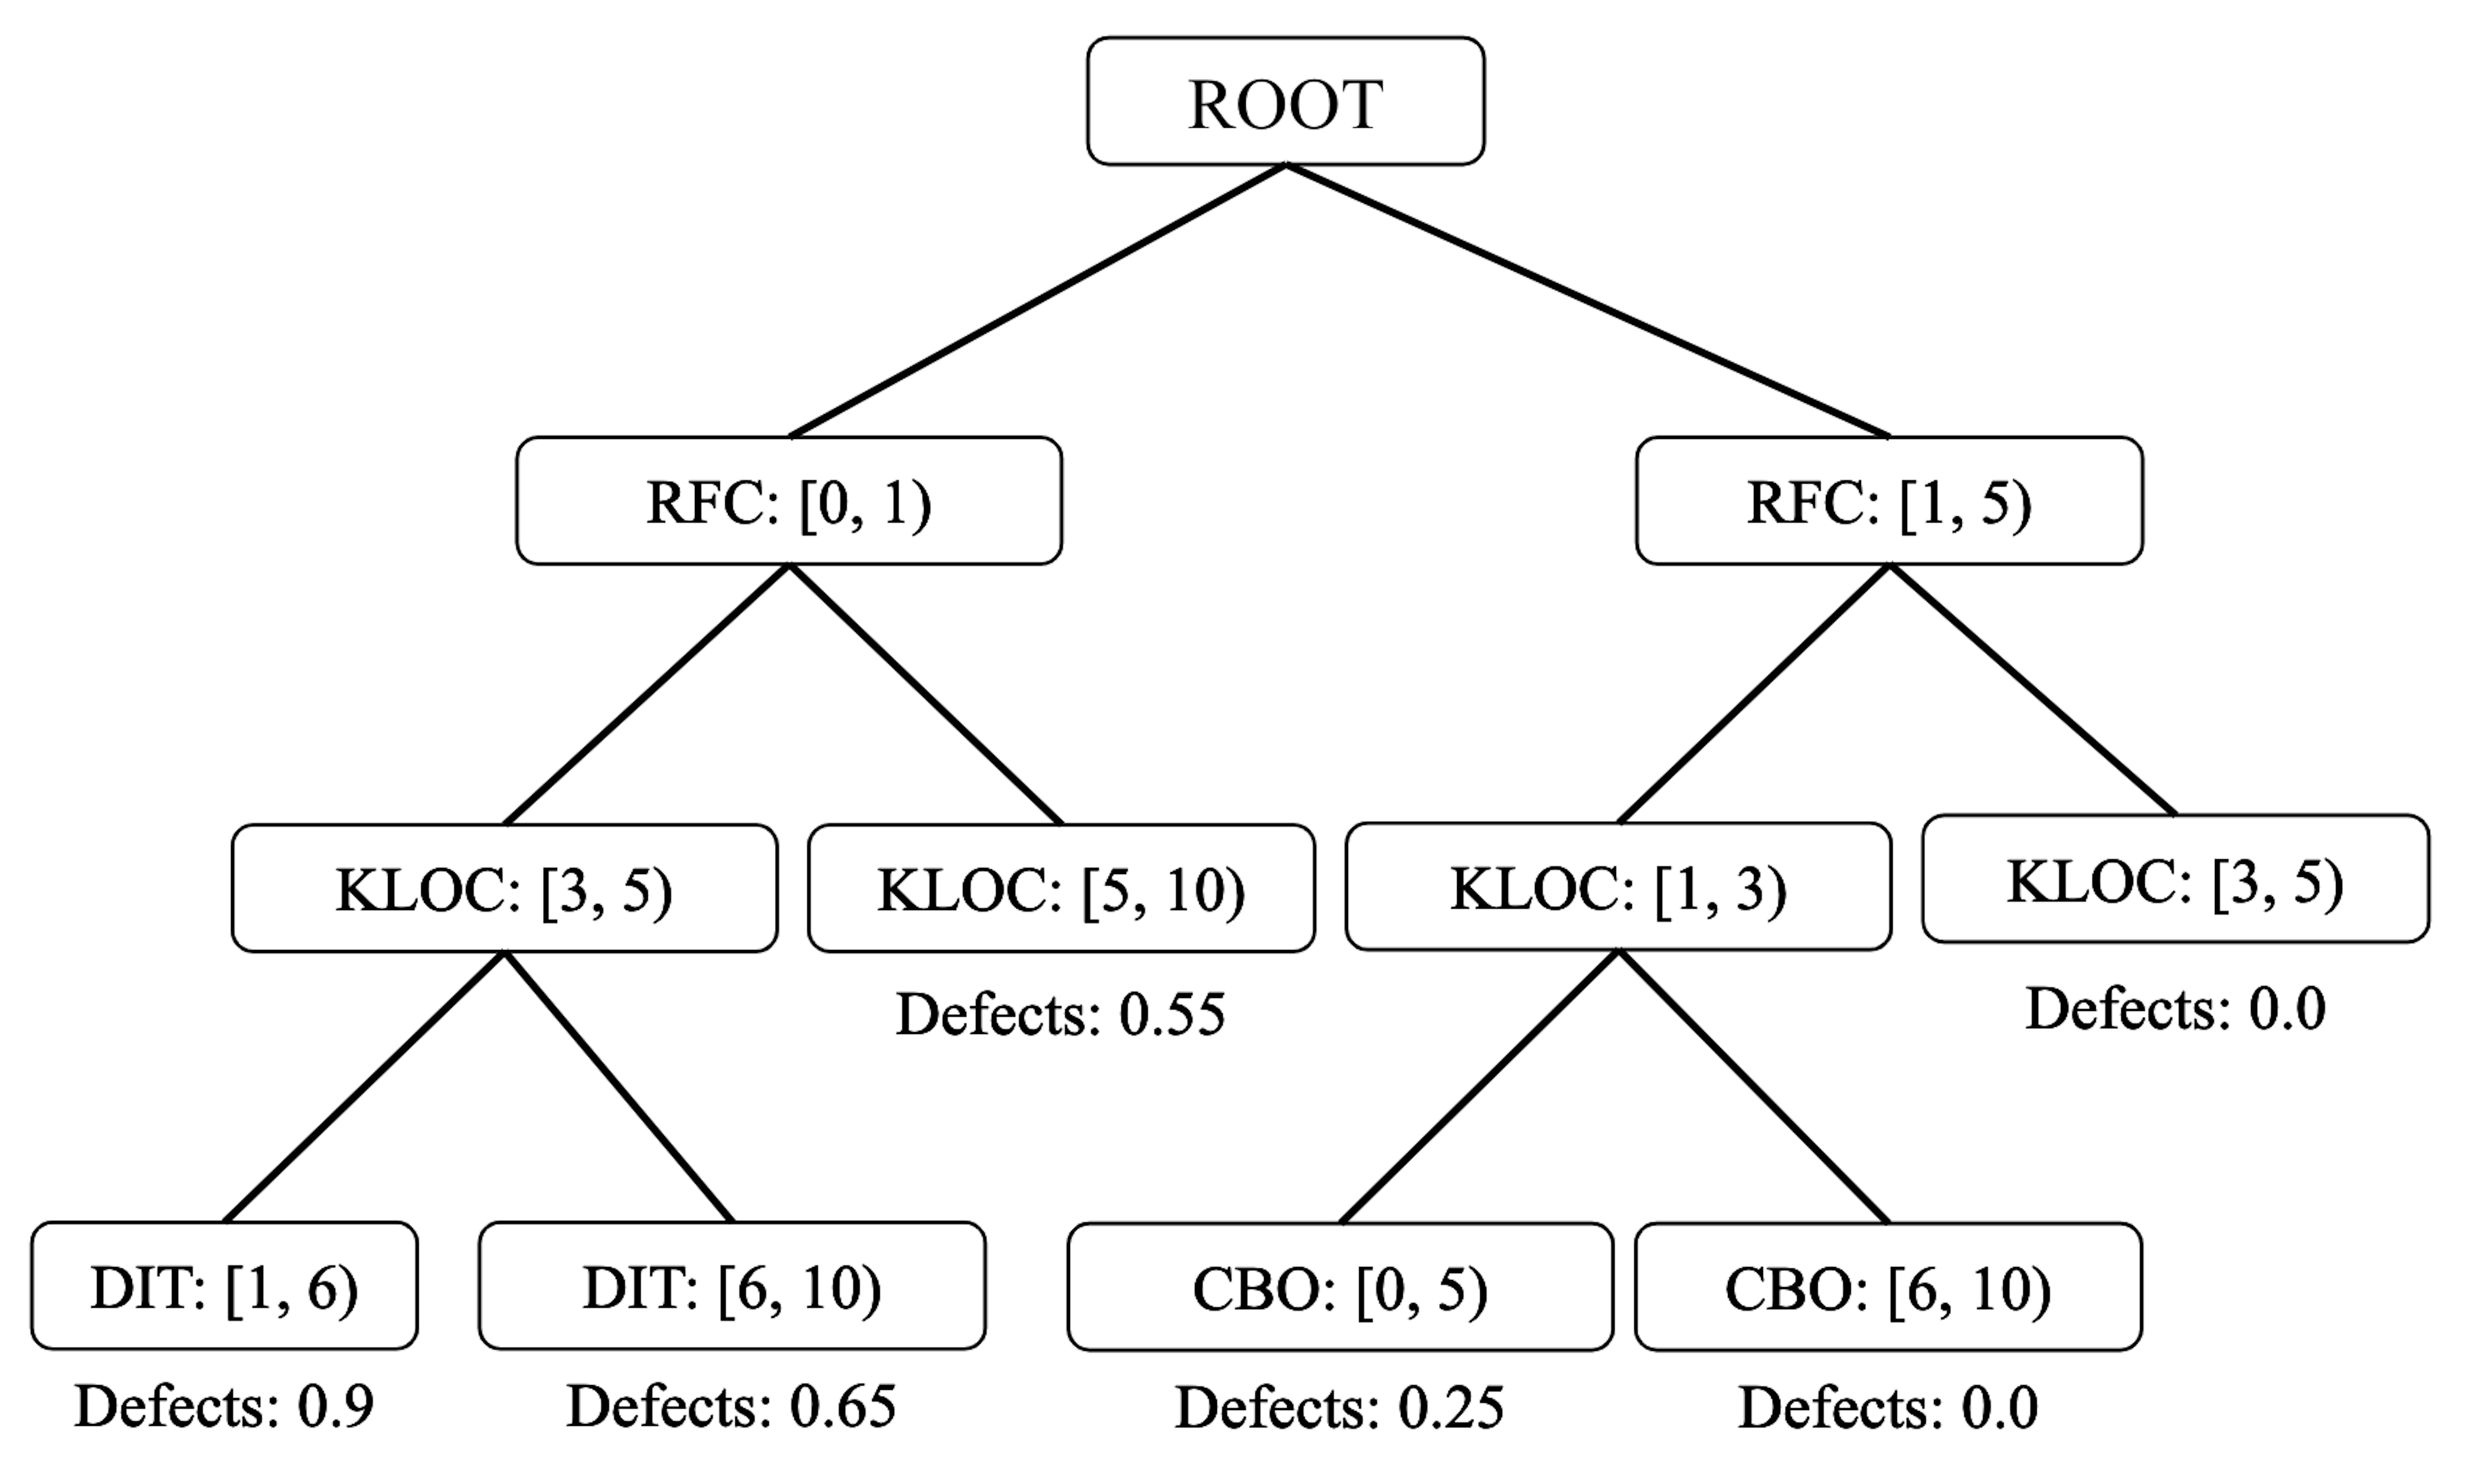
\includegraphics[width=\linewidth]{dtree_fig.png}
    \label{fig:sample_figure}
\end{minipage}
\begin{minipage}[c]{\linewidth}
\centering
(a)~Decision Tree Algorithm\hspace{0.3\linewidth}(b)~Example decision tree
\end{minipage}
\end{minipage}
\end{minipage}\vspace{0.4em}
\bigstrut\\\hline\vspace{-0.5em}
\fig{xtree}.C: For ever test instance, we pass it down the decision tree constructed in \fig{xtree}.B. The node it lands is called the ``start''. Next we find all the ``end'' nodes in the tree, i.e., those which have the lowest likelihood of defects (labeled in \colorbox{black}{{\color{white} black}} below). Finally, perform a random-walk to get from ``start'' to ``end''. We use the mined itemsets from \fig{xtree}.A to guide the walk. When presented with multiple paths, we pick the one which has the largest overlap with the frequent items. e.g., in the below example, we would pick path (b) over path (a).\\[-0.25cm]
\begin{minipage}[c]{\textwidth}
\subfloat[][]{
    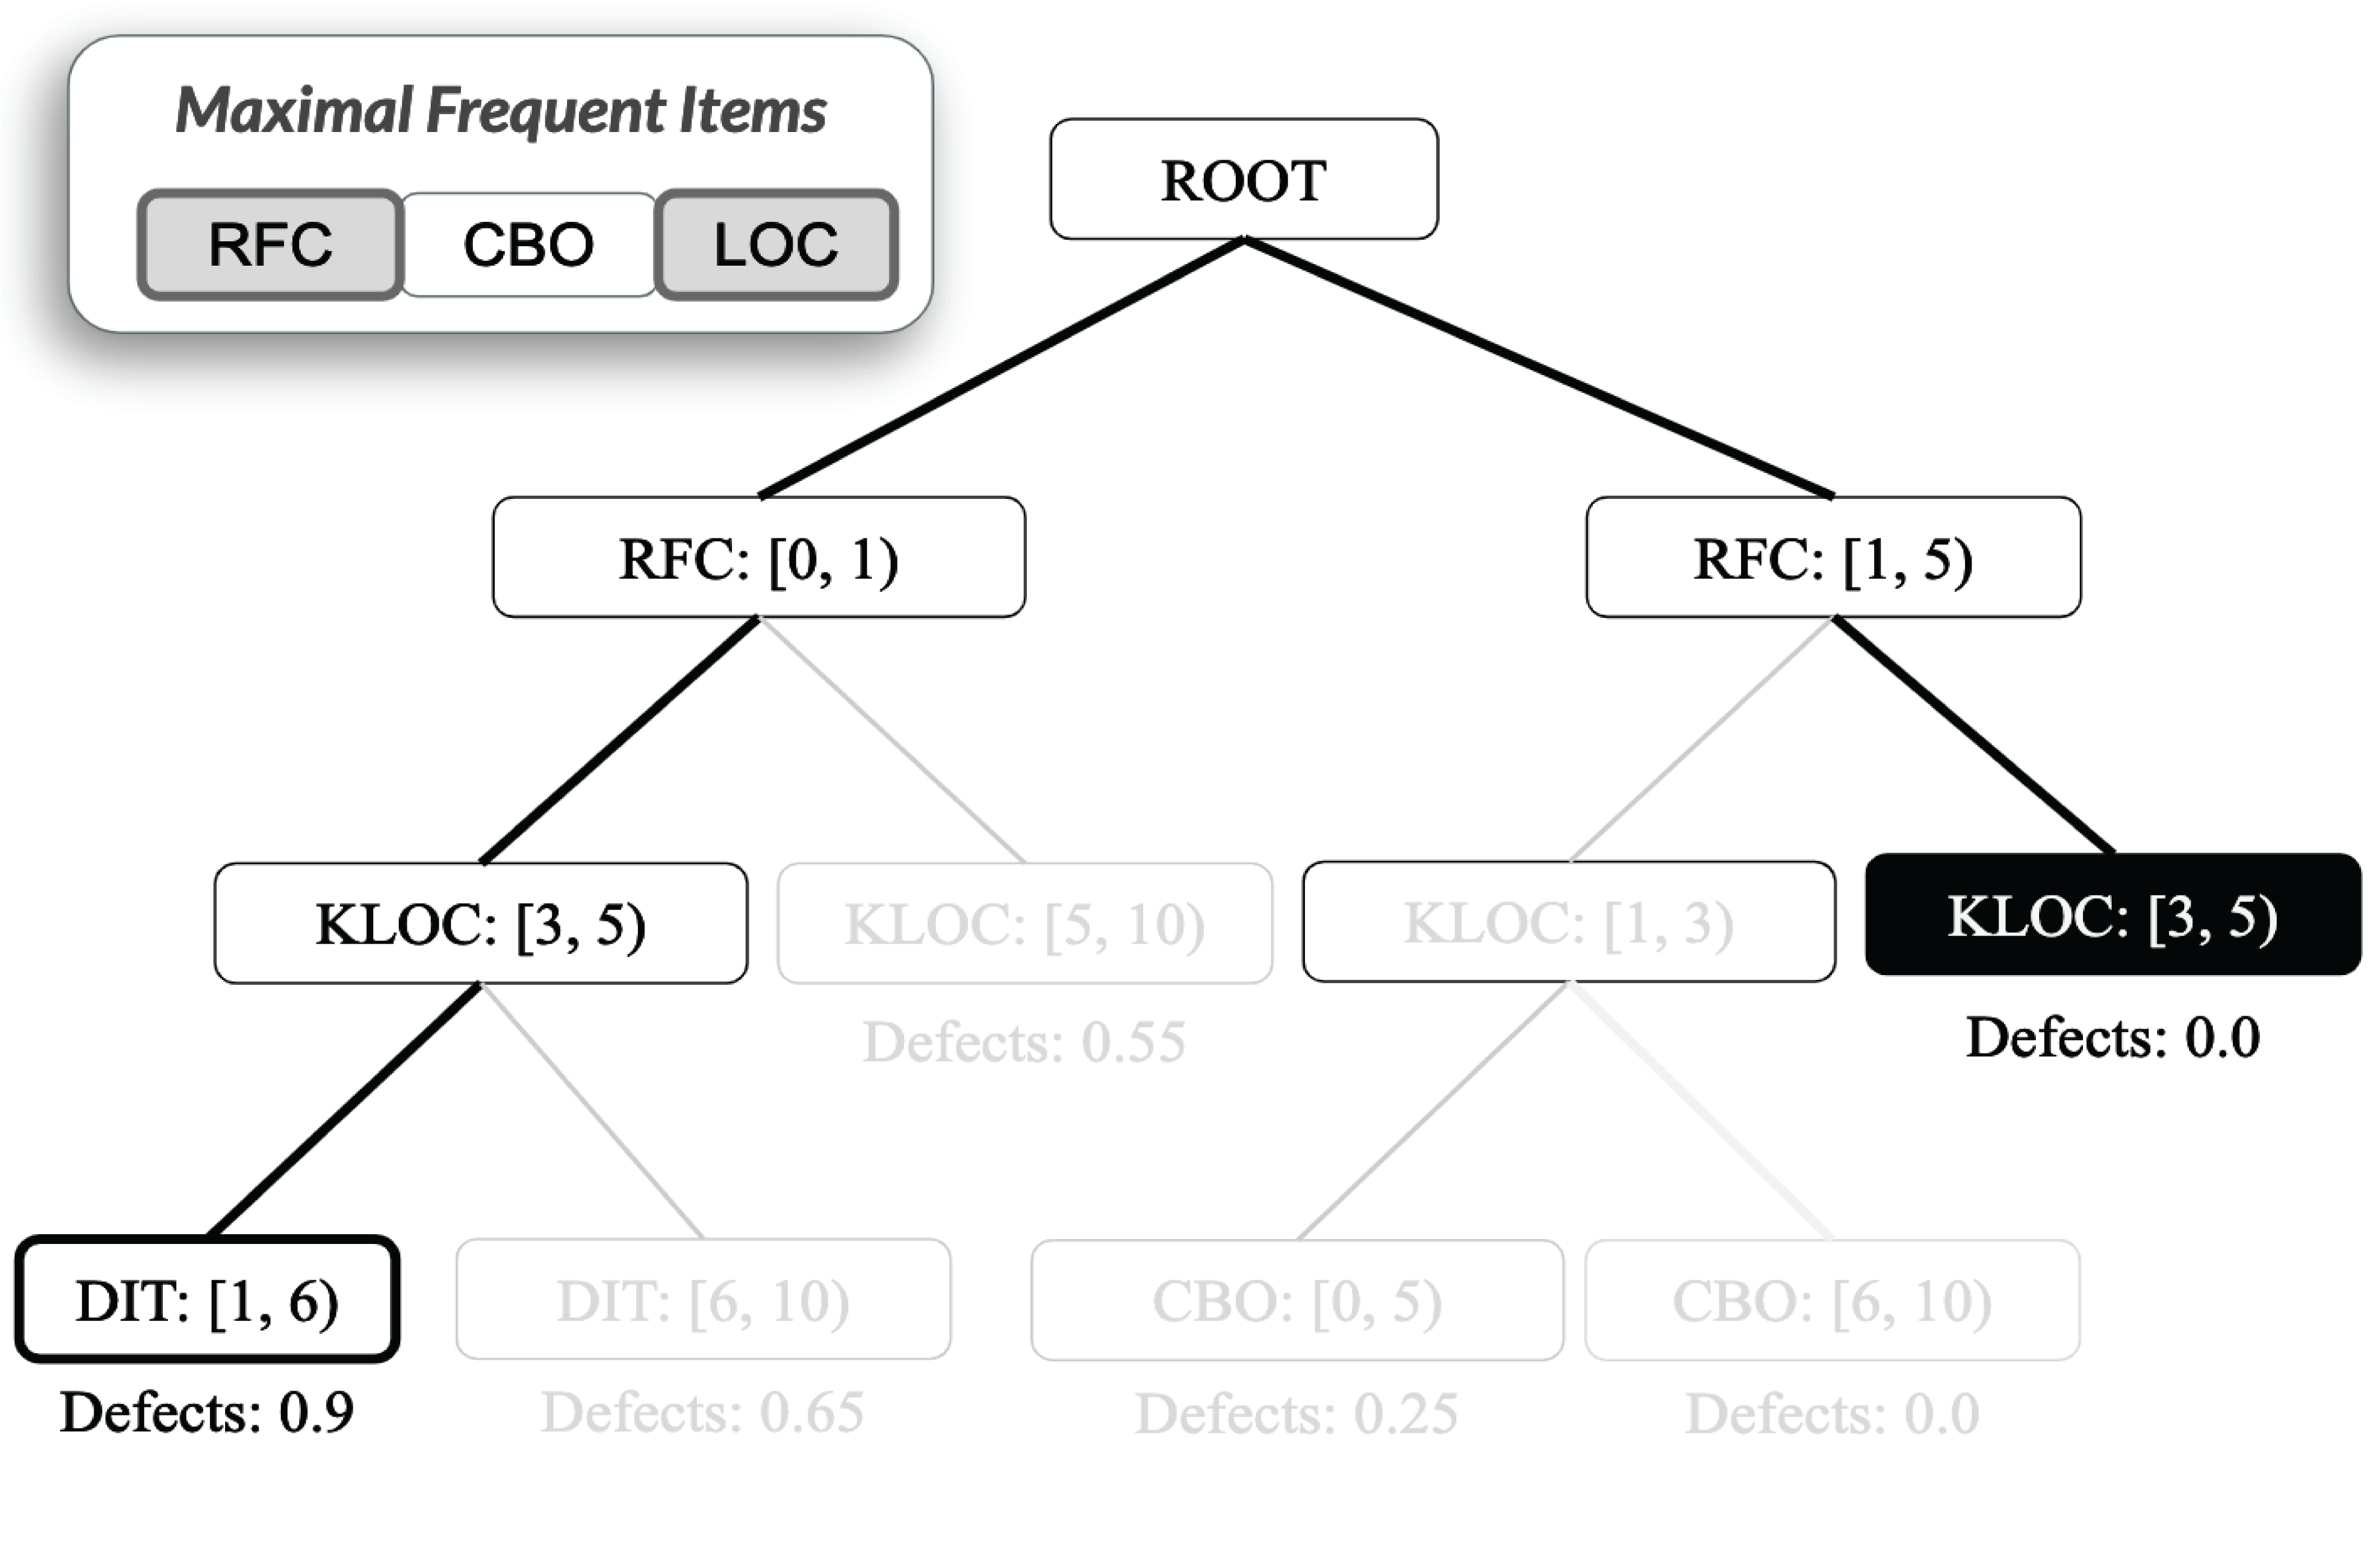
\includegraphics[width=0.5\linewidth]{p3_2.png}
}
\subfloat[][]{
    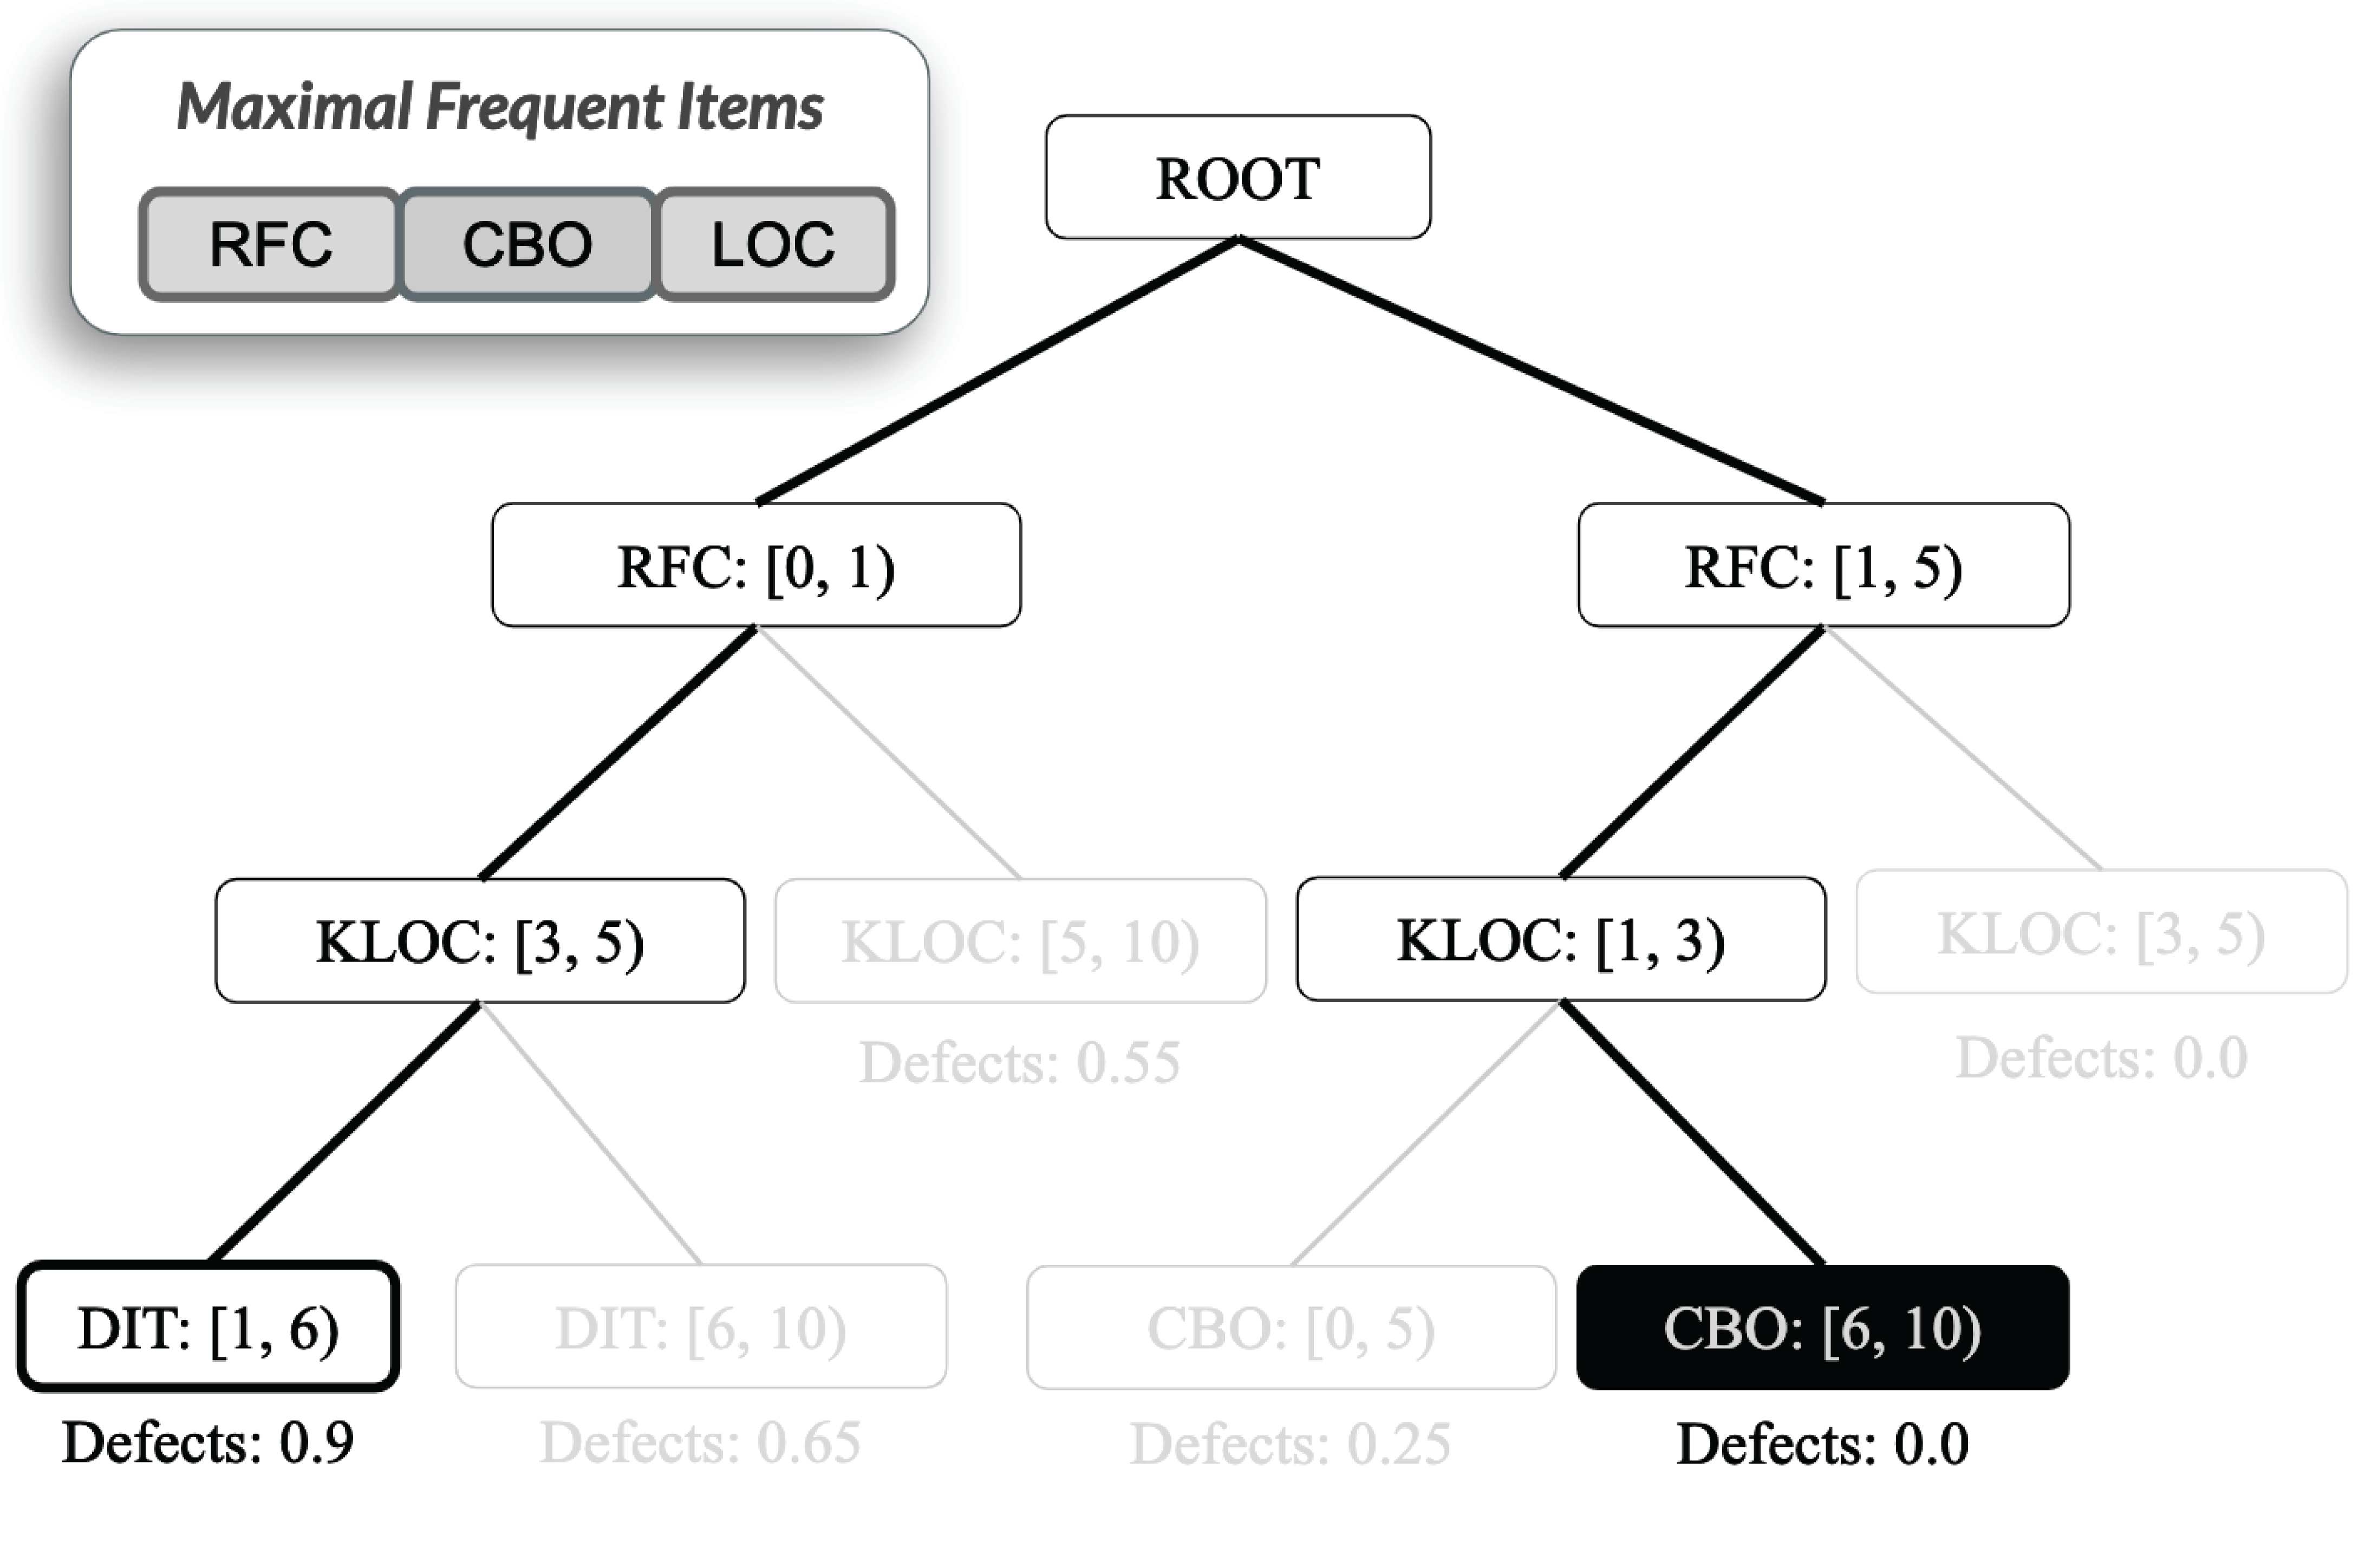
\includegraphics[width=0.5\linewidth]{p3_3.png}
}
\end{minipage}\bigstrut\\\hline
\end{tabular}}
\caption{XTREE Framework}
\label{fig:xtree}
\end{figure}